\chapter{SysML and Scade}
\label{sec:sysML-Scade}

\begin{todo_comment}
Description of the approach by Uwe Steinke.
\end{todo_comment}

Diagram \ref{fig:SysML_SCADE_Toolchain} illustrates the most important components and operational relationships of a system and software modelling toolchain based on SysML, Papyrus, SCADE and Eclipse. 
All components and links shown with solid lines are available, while the dashed ones are intended to be implemented within the openETCS project. 


\begin{figure}[htbp]
	\centering
		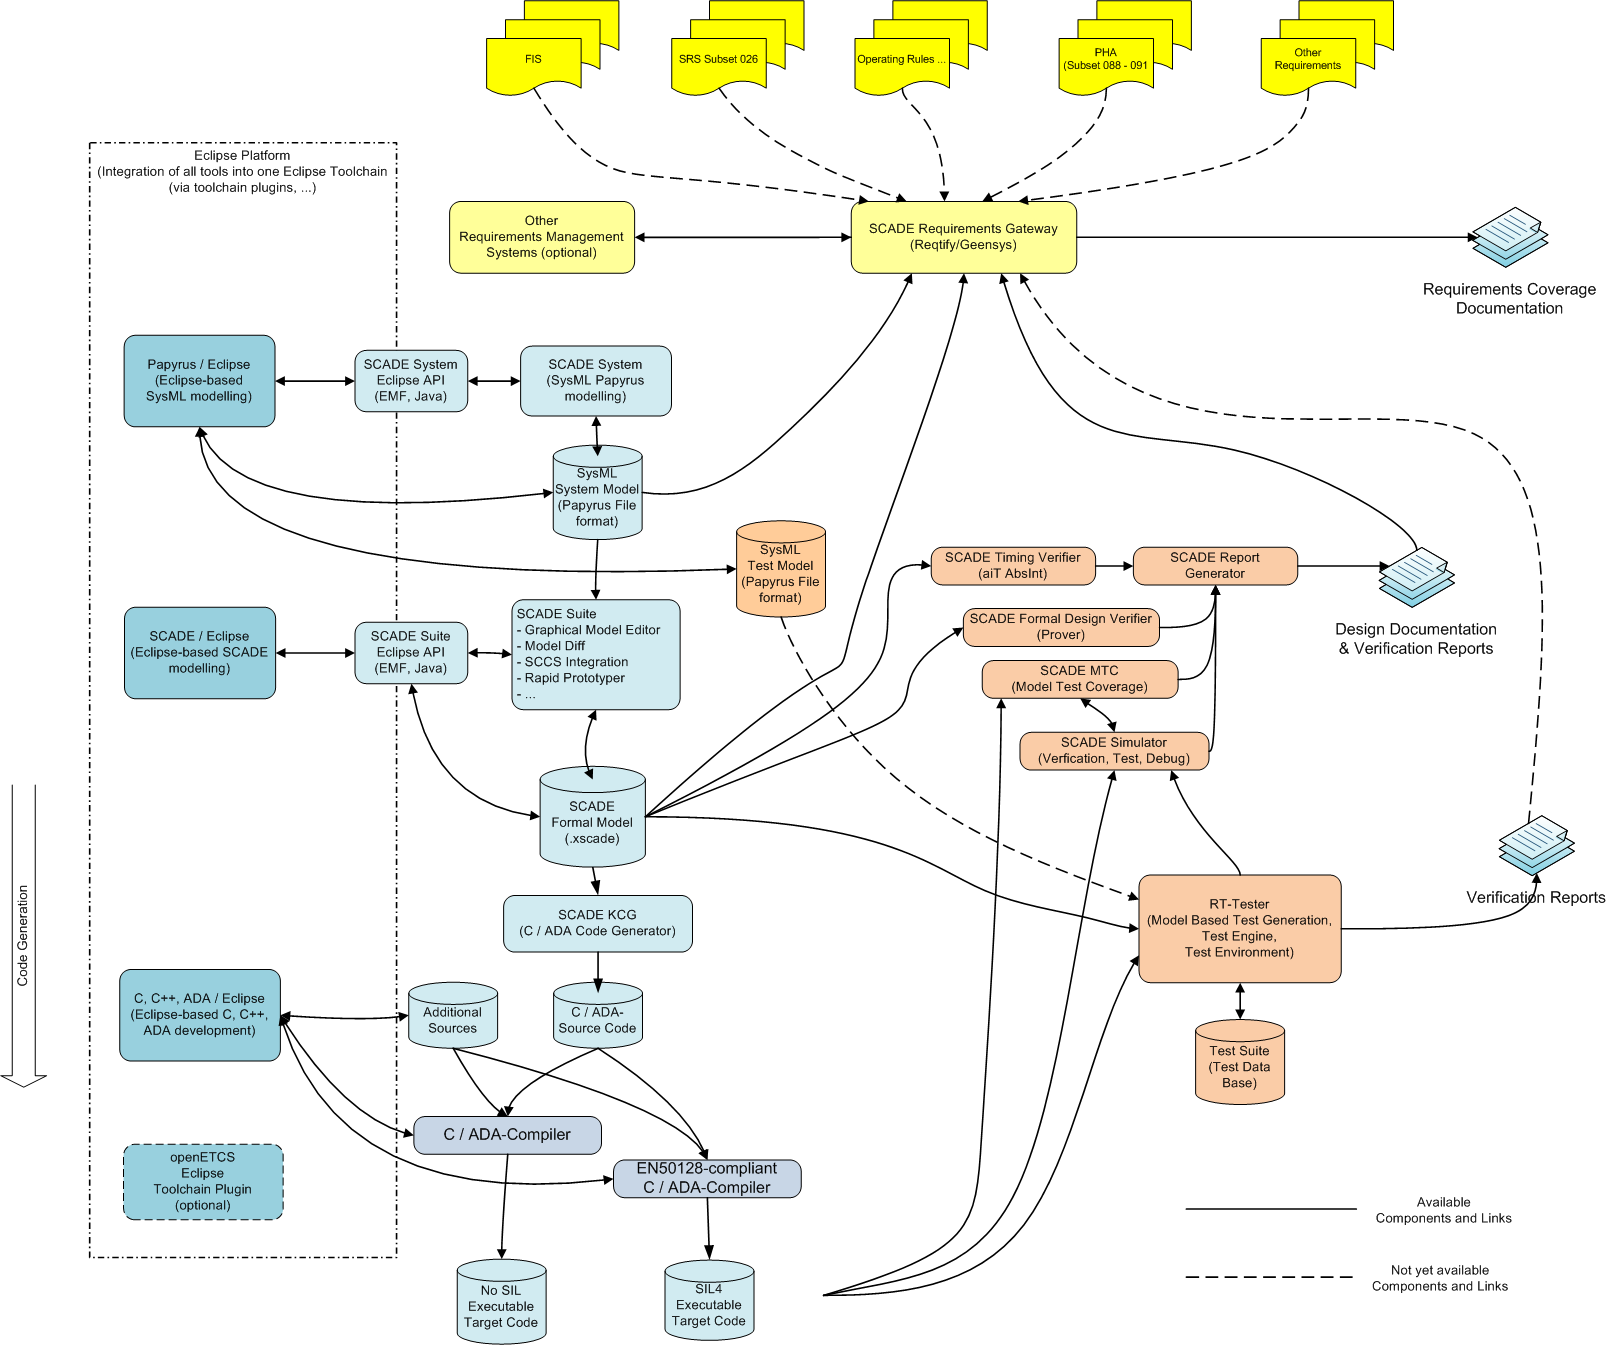
\includegraphics[width=1.10\textwidth]{images/SysML_SCADE_Toolchain.png}
	\caption{SysML SCADE Toolchain}
	\label{fig:SysML_SCADE_Toolchain}
\end{figure}


The diagram colors are chosen related to the colors in \ref{fig:main_process}: 

\begin{itemize}
	\item Requirements and requirements management components in yellow
	\item "Blue" openETCS design process ( see \ref{fig:main_process}) elements in light and dark blue
	\item Eclipse is painted dark blue
	\item Verification elements in red
\end{itemize}

Within the following paragraphs and subsections a short description of this approach will be given by walking through the tool chain and the design process. 

\subsection{Requirements management}
\label{sec:RequirementsManagement}

The SCADE Requirements Management Gateway is based on Reqtify from Geensoft / Dassault Systems and serves to collect and link all requirements from the openETCS input documents and related objects as design und verification documents, model and source code artefacts, test cases, test protocols etc. It supports impact analyses and generates requirements traceability and requirements coverage reports. 
If needed for the openETCS process, it can be complemented with other requirement management systems and already comes with interfaces to these. 


\subsection{Semiformal System and Subsystem Modelling with SCADE System / Papyrus}
\label{sec:SemiformalModelling}

SCADE System is an integration of Papyrus into the SCADE IDE intended for SysML system modelling. It allows to modelize the interactions and hierarchical dependencies between the various parts of a complex system through design elements representing functions, data and interfaces. 
 
The idea is to model system structures, data types / data dictionaries, inputs, outputs, interfaces and relationships between blocks with SysML and transfer it to native SCADE for behavioral modelling automatically. Since Papyrus and SCADE System are using the same file formats, there is no prevention of using all SysML capabilities that Papyrus supports, but in this case without automatic transfer to native SCADE. 

SCADE System supports SysML Block Definition Diagrams (BDD) and	Internal Block Diagrams (IBD).


\subsection{Formal Modelling with SCADE Suite}
\label{sec:FormalModellingwithSCADESuite}

SCADE Suite integrates all modelling, verifation and supporting SCADE tools under the roof of the SCADE IDE. The components relevant for descending part of the development "`V"' process are

\begin{itemize}
	\item SCADE Suite Editor (Graphical and textual modelling)
	\item SCADE Requirements Gateway Integration (Linking of model artefacts with requirements)
	\item SCADE Model Check (model syntax check)
	\item SCADE Model Diff (model comparison)
	\item SCADE Simulator (graphical debugging, simulation and testing) 
	\item SCADE Rapid Prototyper (quick control and display elements for rapid prototyping, optional)
	\item SCADE Code Generator KCG (C / ADA code generation)
	\item SCADE Reporter ( (Design) report generator)
\end{itemize}

The most important tools for modelling are editor and code generator. The others mentioned are mainly verification tools, but very useful and practically indespensible for agile development.

At least, to cover all elements of the "blue" design process in \ref{fig:main_process} a C / C++ / ADA compiler is required. 
For building not safety-relevant executables any C-Compiler (gnu c, ...) is suitable, for safety relevant executables the compiler must be compliant with EN50128.   

\subsection{Model Verification}
\label{sec:SysML_SCADE_ModelVerification}

Will be completed soon. 

\section{Description of the approach for OpenETCS design process}

\begin{todo_comment}
How the proposed approach covers all "blue" design process ( see \ref{fig:main_process}) ?
\end{todo_comment}

The approach as specified in the previous subsections (Chapt. A0) (insert ref xxx) covers all elements of the "blue" design process ( see \ref{fig:main_process}) 
by using the SCADE tool chain including requirements management, semiformal system and formal subsystem/software modelling, code and executable generation. 
An Eclipse integration is provided (see following Chapt. xxx ). 

\section{Integration of the approach with SysML/Papyrus}

\begin{todo_comment}
How the proposed approach can be integrated with the SysML/ Papyrus selected for the high level of design process ?
\end{todo_comment}

Because SCADE System is an integration of Papyrus into the SCADE IDE and SCADE System uses Papyrus file formats, the integration with SysML / Papyrus is available.
A thrilling question for the openETCS process might be, if and - if yes - which of the artefacts on system level should be modelled with SysML, that can not be transferred to native SCADE automatically. 

\section{Integration of the approach with Eclipse}

\begin{todo_comment}
How the proposed approach can be integrated with the Eclipse, selected as platform for OpenETCS tool chain ?
\end{todo_comment}

Most of the the SCADE tools can be run and controlled via command line and/or via automation interfaces. 

SCADE System (SysML modelling) and SCADE Suite (SCADE modelling) already come with Eclipse API plugins based on EMF. These enable to access (read and modify) the model project information, meta and model data from within Eclipse. 
The plugins additionally display the model structure, but they don't show the model graphic in Eclipse. 

If graphical modelling should be done within Eclipse, this has to be implemented by openETCS. It is in doubt, if the effort for this activity would be applicable; without any effort, the SCADE editor should be used instead. 
 
Nevertheless, the provided Eclipse integration is worthwile to supply all openETCS users, that are not directly working on the SCADE models, with an integrated Eclipse tool chain. 
The idea of such an integration is to have one build tool chain, that starts and runs an openETCS executable build process with one button click beginning from all (heterogeneous) sources and performing all necessary model transformations, code and executable generation. 
This could be achieved with an "`openETCS Eclipse Tool Chain Plugin"', implemented as part of the openETCS project with the goals ease-of-use and convenience. 

In summary, an Eclipse integration is available. An optional "`openETCS Eclipse Tool Chain Plugin"' could improve the convenience for openETCS tool chain users. 


\section{Benefits versus OpenETCS requirements}

\begin{todo_comment}
Discuss the benefits in regards of OpenETCS requirements and expected results.
\end{todo_comment}

The most important benefit of the SysML/SCADE approach is its seamless integration, completeness, maturity and qualification for safety critical development: it covers almost all aspects of the openETCS process and lets expect to fill gaps with manageable effort.    

Therefore, the modelling work for openETCS can begin immediately. 

\section{Shortcommings versus OpenETCS requirements}

\begin{todo_comment}
Discuss the shortcommings in regards of OpenETCS requirements and expected results.
\end{todo_comment}

The main drawback of the approach: it is mainly not open Source. 

\section{On going work for openETCS project}

Will be completed soon.

\begin{todo_comment}
Which are the elements to clarify, to specify or to develop, in order the approach suit the openETCS process ?

How can we evaluate and plan this work ?

which skills is needed ?
\end{todo_comment}

\section{Conclusion and other comments}
